% !TEX root = paper-graphnet.tex

\section{Experiments}
\label{sec:exp}

We test the performance of \name\ on three benchmark tasks: (i) classifying academic papers into different subjects using the Web of Science
citation dataset, (ii) classifying Reddit posts as belonging to different communities, and (iii) classifying protein functions across various biological protein-protein interaction (PPI) graphs. Sections \ref{sec:evolving} and \ref{sec:ppi} summarize the datasets, and the supplementary material contains additional information.
In all these experiments, we perform predictions on nodes that are not seen during training, and, in the case of the PPI dataset, we test on entirely unseen graphs. 

\xhdr{Experimental set-up}
To contextualize the empirical results on our inductive benchmarks, we compare against four baselines: 
a random classifer, a logistic regression feature-based classifier (that ignores graph structure), the DeepWalk algorithm \cite{perozzi2014deepwalk} as a representative factorization-based approach, and a
concatenation of the raw features and DeepWalk embeddings.
We also compare four variants of \name\ that use the different aggregator functions (Section \ref{sec:aggs}).
Since, the ``convolutional'' variant of \name\ is an extended, inductive version of Kipf et al's semi-supervised GCN \cite{kipf2016semi}, we term this variant \name-GCN.
We test unsupervised variants of \name\, trained according to the loss in Equation \eqref{eq:neg}, as well as supervised variants that are trained directly on classification cross-entropy loss.
For all the \name\ variants we used rectified linear units as the non-linearity and set $K=2$ with neighborhood sample sizes $S_1=25$ and $S_2=10$ (see Section \ref{sec:sensitivity} for sensitivity analyses).

For the Reddit and citation datasets, we use ``online'' training for DeepWalk as described in Perozzi et al.~\cite{perozzi2014deepwalk}, where we run a new round of SGD optimization to embed the new test nodes before making predictions (see the Appendix for details).
In the multi-graph setting, we cannot apply DeepWalk, since the embedding spaces generated by running the DeepWalk algorithm on different disjoint graphs can be arbitrarily rotated with respect to each other (Appendix \ref{sec:rotational}). 



All models were implemented in TensorFlow \cite{abadi2016tensorflow} with the Adam optimizer \cite{kingma2014adam} (except DeepWalk, which performed better with the vanilla gradient descent optimizer). 
We designed our experiments with the goals of (i) verifying the improvement of \name\ over the baseline approaches (i.e., raw features and DeepWalk) and (ii) providing a rigorous comparison of the different \name\ aggregator architectures. 
In order to provide a fair comparison, all models share an identical implementation of their minibatch iterators, loss function and neighborhood sampler (when applicable). 
Moreover, in order to guard against unintentional ``hyperparameter hacking'' in the comparisons between \name\ aggregators, we sweep over the same set of hyperparameters for all \name\ variants (choosing the best setting for each variant according to performance on a validation set). 
The set of possible hyperparameter values was determined on early validation tests using subsets of the citation and Reddit data that we then discarded from our analyses. 
The appendix contains further implementation details.\footnote{Code and links to the datasets:  \url{http://snap.stanford.edu/graphsage/}}




\subsection{Inductive learning on evolving graphs: Citation and Reddit data}
\label{sec:evolving}

\begin{table}[t!]
\centering
\caption{Prediction results for the three datasets (micro-averaged F1 scores). Results for unsupervised and fully supervised \name\ are shown. Analogous trends hold for macro-averaged scores.}
\label{tab:main_results}
{\small
\begin{tabular}{lcccccc}
\toprule
&\multicolumn{2}{c}{Citation}& \multicolumn{2}{c}{Reddit} & \multicolumn{2}{c}{PPI} \\
\cmidrule(r{1em}l{1em}){2-3}  \cmidrule(r{1em}l{1em}){4-5} \cmidrule(r{1em}l{1em}){6-7}
Name & Unsup. F1 &  Sup. F1 & Unsup. F1 & Sup. F1 &  Unsup. F1 & Sup. F1\\
\midrule
Random & 0.206 & 0.206 & 0.043 & 0.042 & 0.396 & 0.396 \\
Raw features & 0.575 & 0.575 & 0.585 & 0.585 & 0.422 & 0.422 \\
DeepWalk & 0.565 &  0.565 & 0.324 & 0.324 &  --- & --- \\\vspace{3pt}
DeepWalk + features & 0.701 &   0.701 & 0.691 & 0.691 & --- & --- \\
\name-GCN & 0.742 & 0.772 & {\bf 0.908} &  0.930 & 0.465 &  0.500\\
\name-mean & 0.778 & 0.820 & 0.897 &  0.950 & 0.486 & 0.598 \\
\name-LSTM & 0.788 & 0.832 & {\bf 0.907} & {\bf 0.954} & 0.482 &  {\bf 0.612}\\
\name-pool & {\bf 0.798} & {\bf 0.839} & 0.892 & 0.948 &  {\bf 0.502} & 0.600\\
\midrule
\% gain over feat. & 39\% & 46\% & 55\% & 63\% & 19\% & 45\%\\
\bottomrule
\end{tabular}
}
\end{table}
\begin{figure}
\vspace{-10pt}
\begin{subfigure}[t]{0.48\textwidth}
\centering
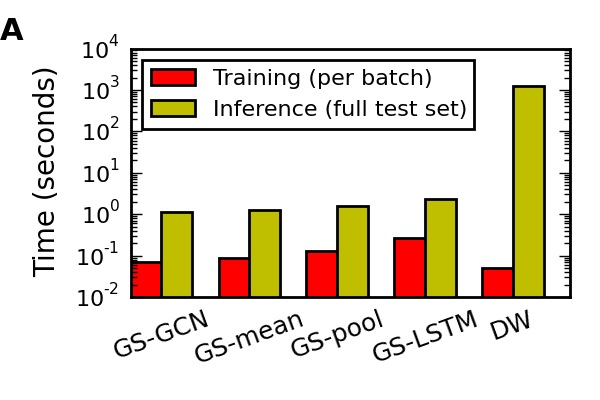
\includegraphics[width=0.99\textwidth]{timing.png}
\end{subfigure}
\begin{subfigure}[t]{0.52\textwidth}
\centering
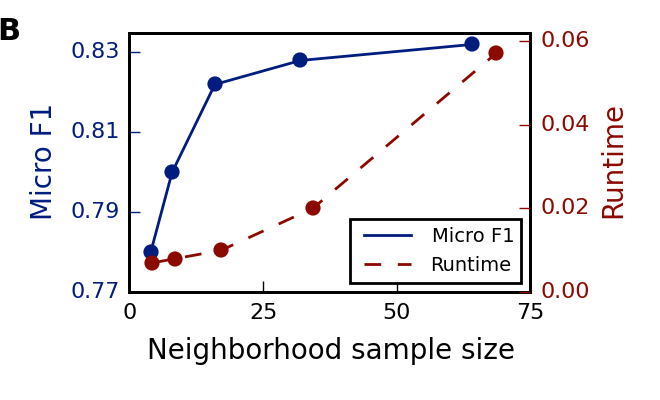
\includegraphics[width=0.99\textwidth]{neigh_tradeoff.png}
\end{subfigure}
\caption{\textbf{A}: Timing experiments on Reddit data, with training batches of size 512 and inference on the full test set (79,534 nodes). \textbf{B}: Model performance with respect to the size of the sampled neighborhood, where the ``neighborhood sample size'' refers to the number of neighbors sampled at each depth for $K=2$ with  $S_1=S_2$ (on the citation data using \name-mean). }
%\vspace{-15pt}
\label{fig:time_and_noise}
\end{figure}

Our first two experiments are on classifying nodes in evolving information graphs, a task that is especially relevant to high-throughput production systems, which constantly encounter unseen data. 

\xhdr{Citation data}
Our first task is predicting paper subject categories on a large citation dataset. 
We use an undirected citation graph dataset derived from the Thomson Reuters Web of Science Core Collection, corresponding to all papers in six biology-related fields for the years 2000-2005.
The node labels for this dataset correspond to the six different field labels. 
In total, this is dataset contains 302,424 nodes with an average degree of 9.15.
We train all the algorithms on the 2000-2004 data and use the 2005 data for testing (with 30\% used for validation). 
For features, we used node degrees and processed the paper abstracts according Arora et al.'s~\cite{arora2017simple} sentence embedding approach, with 300-dimensional word vectors trained using the GenSim word2vec implementation \cite{rehurek_lrec}.

\xhdr{Reddit data}
In our second task, we predict which community different Reddit posts belong to. 
Reddit is a large online discussion forum where users post and comment on content in different topical communities. 
We constructed a graph dataset from Reddit posts made in the month of September, 2014. 
The node label in this case is the community, or ``subreddit'', that a post belongs to.  
We sampled 50 large communities and built a post-to-post graph, connecting posts if the same user comments on both. 
In total this dataset contains 232,965 posts with an average degree of 492.
We use the first 20 days for training and the remaining days for testing (with 30\% used for validation).  
For features, we use off-the-shelf 300-dimensional GloVe CommonCrawl word vectors \cite{pennington2014glove}; for each post, we concatenated (i) the average embedding of the post title, (ii) the average embedding of all the post's comments (iii) the post's score, and (iv) the number of comments made on the post. 

The first four columns of Table \ref{tab:main_results} summarize the performance of \name\, as well as the baseline approaches on these two datasets.
We find that \name\ outperforms all the baselines by a significant margin, and the trainable, neural network aggregators provide significant gains compared to the GCN approach. 
For example, the unsupervised variant \name-pool outperforms the concatenation of the DeepWalk embeddings and the raw features by 13.8\% on the citation data and 29.1\% on the Reddit data, while the supervised version provides a gain of 19.7\% and 37.2\%, respectively. 
Interestingly, the LSTM based aggregator shows strong performance, despite the fact that it is designed for sequential data and not unordered sets. 
Lastly, we see that the performance of unsupervised \name\ is reasonably competitive with the fully supervised version, indicating that our framework can achieve strong performance without task-specific fine-tuning. 
 
\subsection{Generalizing across graphs: Protein-protein interactions}\label{sec:ppi}

We now consider the task of generalizing across graphs, which requires learning about node roles rather than community structure. 
We classify protein roles---in terms of their cellular functions from gene ontology---in various
protein-protein interaction (PPI) graphs, with each graph corresponding to a different human tissue \cite{zitnik2017tissue}.
We use positional gene sets, motif gene sets and immunological signatures as features and gene
ontology sets as labels (121 in total), collected from the Molecular Signatures Database \cite{subramanian2005gene}.
The average graph contains 2373 nodes, with an average degree of 28.8.
We train all algorithms on 20 graphs and then average prediction F1 scores on two test graphs (with two other graphs used for validation). 

The final two columns of Table \ref{tab:main_results} summarize the accuracies of the various approaches on this data.
Again we see that \name\ significantly outperforms the baseline approaches, with the LSTM- and pooling-based aggregators providing substantial gains over the mean- and GCN-based aggregators.\footnote{Note that in very recent follow-up work Chen and Zhu \cite{chen2017stochastic} achieve superior performance by optimizing the \name\ hyperparameters specifically for the PPI task and implementing new training techniques (e.g., dropout, layer normalization, and a new sampling scheme). We refer the reader to their work for the current state-of-the-art numbers on the PPI dataset that are possible using a variant of the \name\ approach.} 


\subsection{Runtime and parameter sensitivity}\label{sec:sensitivity}

Figure \ref{fig:time_and_noise}.A summarizes the training and test runtimes for the different approaches. 
The training time for the methods are comparable (with \name-LSTM being the slowest). 
However, the need to sample new random walks and run new rounds of SGD to embed unseen nodes makes DeepWalk $100\text{-}500\times$ slower at test time. 

For the \name\ variants, we found that setting $K=2$ provided a consistent boost in accuracy of around $10\text{-}15\%$, on average, compared
to $K=1$; however, increasing $K$ beyond 2 gave marginal returns in performance ($0\text{-}5\%$)
while increasing the runtime by a prohibitively large factor of $10\text{-}100{\times}$, depending
on the neighborhood sample size.
We also found diminishing returns for sampling large neighborhoods (Figure
\ref{fig:time_and_noise}.B).
Thus, despite
the higher variance induced by sub-sampling neighborhoods, \name\ is still able to maintain strong predictive accuracy, while significantly improving the runtime. 

\subsection{Summary comparison between the different aggregator architectures}\label{sec:sensitivity}

Overall, we found that the LSTM- and pool-based aggregators performed the best, in terms of both average performance and number of experimental settings where they were the top-performing method (Table \ref{tab:main_results}).
To give more quantitative insight into these trends, we consider each of the six different experimental settings (i.e., $\textrm{(3 datasets)} \times (\textrm{unsupervised vs.\ supervised})$) as trials and consider what performance trends are likely to generalize.
In particular, we use the non-parametric Wilcoxon Signed-Rank Test \cite{siegal1956nonparametric} to quantify the differences between the different aggregators across trials, reporting the $T$-statistic and $p$-value where applicable. 
Note that this method is rank-based and essentially tests whether we would expect one particular approach to outperform another in a new experimental setting.
Given our small sample size of only 6 different settings, this significance test is somewhat underpowered; nonetheless, the $T$-statistic and associated $p$-values are useful quantitative measures to assess the aggregators' relative performances. 

We see that LSTM-, pool- and mean-based aggregators all provide statistically significant gains over the GCN-based approach ($T=1.0$, $p=0.02$ for all three). 
However, the gains of the LSTM and pool approaches over the mean-based aggregator are more marginal ($T=1.5$, $p=0.03$, comparing LSTM to mean; $T=4.5$, $p=0.10$, comparing pool to mean).
There is no significant difference between the LSTM and pool approaches ($T=10.0$, $p=0.46$). 
However, \name-LSTM is significantly slower than \name-pool (by a factor of ${\approx}2{\times}$), perhaps giving the pooling-based aggregator a slight edge overall. 


\section{Theoretical analysis}\label{sec:theory}

In this section, we probe the expressive capabilities of \name\ in order to 
provide insight into how \name\ can learn about graph structure, even though it is inherently based on features. 
As a case-study, we consider whether \name\ can learn to predict the clustering coefficient of a node, i.e., the proportion of triangles that are closed within the node's 1-hop neighborhood \cite{watts1998collective}.  The clustering coefficient is a popular  measure of how clustered a node's local neighborhood is, and it serves as a building block for many more complicated structural motifs \cite{benson2016higher}. We can show that Algorithm \ref{alg:basic} is capable of approximating clustering coefficients to an arbitrary degree of precision:

\begin{theorem}\label{thm:main}
Let $\mb{x}_v \in U, \forall v \in \mathcal{V}$ denote the feature inputs for Algorithm \ref{alg:basic} on graph $\mathcal{G}=(\mathcal{V}, \mathcal{E})$, where $U$ is any compact subset of $\mathbb{R}^d$. Suppose that there exists a fixed positive constant $C \in \mathbb{R}^+$ such that $\|\mb{x}_v  - \mb{x}_{v'}\|_2 > C$ for all pairs of nodes. Then we have that $\forall \epsilon > 0$ there exists a parameter setting $\mb{\Theta}^*$ for Algorithm \ref{alg:basic} such that after $K=4$ iterations
$$|{z}_v - c_v| < \epsilon , \forall v \in \mathcal{\V},$$ where $z_v \in \mathbb{R}$ are final output values generated by Algorithm 1 and $c_v$ are node clustering coefficients.\cut{, as defined in \cite{watts1998collective}.}
\end{theorem}

Theorem 1 states that for any graph there exists a parameter setting for Algorithm 1 such that it can approximate clustering coefficients in that graph to an arbitrary precision, if the features for every node are distinct (and if the model is sufficiently high-dimensional). 
The full proof of Theorem 1 is in the Appendix. 
Note that as a corollary of Theorem 1, \name\ can learn about local graph structure, even when the node feature inputs are sampled from an absolutely continuous random distribution (see the Appendix for details).
The basic idea behind the proof is that if each node has a unique feature representation, then we can learn to map nodes to indicator vectors and identify node neighborhoods.
The proof of Theorem 1 relies on some properties of the pooling aggregator, which also provides insight into why \name-pool outperforms the GCN and mean-based aggregators. 